% fig_residual.tex
% Charging residual floor and detection threshold for three correction methods
% Data from TR-13/15: fixed=1.43 pu, pre-fault blind=0.001 pu, voltage=0.001 pu
% Threshold: 0.20 pu -> 0.12 pu -> 0.08 pu
% Grouped bar: residual (orange) + threshold (blue) per method, log y-axis
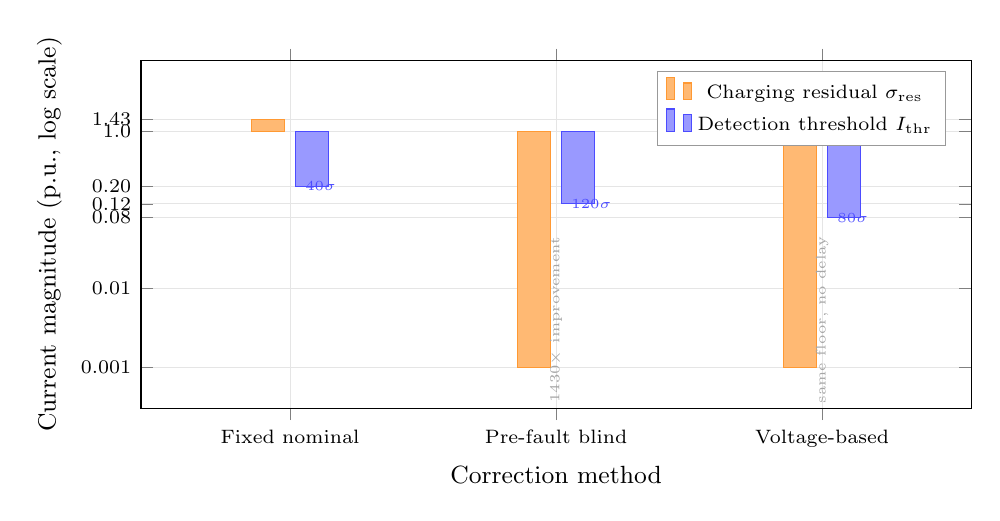
\begin{tikzpicture}
\begin{axis}[
  width=\columnwidth, height=6.0cm,
  ybar=4pt,
  bar width=0.42cm,
  ymode=log,
  xlabel={Correction method},
  ylabel={Current magnitude (p.u., log scale)},
  symbolic x coords={Fixed nominal, Pre-fault blind, Voltage-based},
  xtick=data,
  xticklabel style={font=\scriptsize,align=center,text width=2.6cm},
  ymin=3e-4, ymax=8,
  ytick={0.001,0.01,0.08,0.12,0.20,1.0,1.43},
  yticklabels={0.001,0.01,0.08,0.12,0.20,1.0,1.43},
  yticklabel style={font=\scriptsize},
  grid=both,
  grid style={gray!20,line width=0.3pt},
  label style={font=\small},
  tick label style={font=\scriptsize},
  legend style={at={(0.97,0.97)},anchor=north east,
                font=\scriptsize,fill=white,draw=black!40},
  enlarge x limits=0.28,
  clip=false]

  % Residual floor bars (orange)
  \addplot[fill=orange!55,draw=orange!80] coordinates {
    (Fixed nominal,    1.43)
    (Pre-fault blind,  0.001)
    (Voltage-based,    0.001)
  };
  \addlegendentry{Charging residual $\sigma_{\rm res}$}

  % Detection threshold bars (blue)
  \addplot[fill=blue!40,draw=blue!70] coordinates {
    (Fixed nominal,   0.20)
    (Pre-fault blind, 0.12)
    (Voltage-based,   0.08)
  };
  \addlegendentry{Detection threshold $I_{\rm thr}$}

  % Improvement annotations
  \node[font=\tiny,rotate=90,gray!70]
    at (axis cs:Pre-fault blind, 0.004) {1430$\times$ improvement};
  \node[font=\tiny,rotate=90,gray!70]
    at (axis cs:Voltage-based,   0.004) {same floor, no delay};

  % Noise margin annotations
  \node[font=\tiny,blue!70,right=2pt]
    at (axis cs:Fixed nominal,   0.20) {$40\sigma$};
  \node[font=\tiny,blue!70,right=2pt]
    at (axis cs:Pre-fault blind, 0.12) {$120\sigma$};
  \node[font=\tiny,blue!70,right=2pt]
    at (axis cs:Voltage-based,   0.08) {$80\sigma$};

\end{axis}
\end{tikzpicture}
